%\documentclass[margin=0mm]{standalone}
%\usepackage{tikz}
%\usepackage{pgfplots}
% \pgfplotsset{compat=newest}
%
%
%\usepackage{currfile,hyperxmp}
%\usetikzlibrary{math,calc,matrix,fit,positioning,intersections}
%
%\usepackage{tikz-3dplot}
% 
%\usepackage{xfp}
%\usepackage{amsmath}
%
%\begin{document}
%
%
%


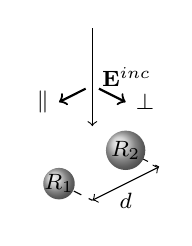
\begin{tikzpicture}
%\useasboundingbox (0,0) rectangle (5,5);
%\draw (11,10) rectangle ++(5,5);


 \begin{axis}[height=24cm,
   axis lines=none,
    xmin=-3.5,
    xmax=3.5,
    ymin=-3.5,
    ymax=3.5,
    zmin=-3.5,
    zmax=5.5,
 %   xtick=\empty,
  %  ytick=\empty,
   % ztick=\empty,
    axis equal , rotate around z=70 ,rotate around x=0 ,
    font=\footnotesize]

\tikzmath{\u=1; \v=2; \w=2;}   

 
  \draw[<-] (0,0,0.5) -- node [right] {$\mathbf{E}^\text{inc}$} (0,0,1.7);

  \draw[->, thick] (0,-0.1,1) -- (0, -0.5, 1) node[right] {$\perp$};
 \draw[->, thick] (-0.1,0 ,1) -- ( -0.5,0, 1) node [left] {$\parallel$};
  

  \draw[dashed] (-0.5, 0,0) --  (-0.5, -0.5, 0);
  \draw[dashed] (0.5, 0,0) --  (0.5, -0.5, 0);
  \draw [<->]  (0.5, -0.5, 0) -- node [below] {$d$} (-0.5, -0.5, 0);


  	\shade [ball color=gray!50!white](-0.5,0,0) circle (2mm) node {$R_1$};
  	\shade [ball color=gray!50!white](0.5,0,0) circle (2.5mm)node {$R_2$};


  \end{axis}

  
  \end{tikzpicture}

%\end{document}

